% it is essential to demonstrate that a proper professional approach was employed

% It should show how the project proposal was further refined and clarified, so that the implementation stage could go smoothly rather than by trial and error.

% You must demonstrate a structured design approach, including high-level design planning, design-for-test, consideration of human factors and systematic evaluation including confidence metrics within your evaluation where appropriate. You should explain how you would show conformance with appropriate legislation, such as that for intellectual property, data protection, human subjects and software licenses such as those for open source. Show that you understand the consequences of your project (or a more fully-formed variant of it) in terms of how it might affect commercial markets, contribute to society and/or the research community.

% Challenging and well-presented background covering Comp Sci topics beyond Part IB.

% Good requirements analysis, justified selection of suitable tools, good engineering approach.

\label{sec:2}

\section{Starting Point}
\label{sec:starting-point}
As noted in the \hyperref[sec:relevant-work]{\textit{Relevant Work}} section, visual SLAM systems are a mature and well-researched subfield of Computer Science with many advanced implementations. To avoid spending the majority of my effort re-implementing a visual SLAM system from scratch, I instead used a \textbf{single-agent} visual SLAM implementation as the starting point for my project. The thinking behind this decision was that it would allow me to focus my efforts on the distributed multi-agent aspect of this project, which I believe is a novel and under-researched aspect of the field.

I chose ORB-SLAM3 as the single agent SLAM system to base my system on top of, as it ranks at the top of benchmarks in a variety of environments \autocite{DBLP:journals/corr/abs-2108-01654} and its researchers released code alongside their paper. I primarily utilized the system's visual odometry (VO) front end and helper functions from the backend to perform operations such as bundle adjustment.

While ORB-SLAM3 is an excellent SLAM system, it is fundamentally a single-agent system with no considerations in place for use in a multi-agent context. As I will expand on in the \hyperref[sec:orb-slam-3]{\textit{ORB-SLAM 3}} section, a significant amount of time and effort was required to understand its extremely large undocumented codebase, especially since an almost complete understanding of its inner workings were needed to both extract and inject map information from the system. In retrospect, using an existing single-agent SLAM system as a foundation may not have saved as much time as I had initially hoped. I spent all of Michaelmas term wrangling with ORB-SLAM's codebase and was not able to begin making proper progress on the distributed aspect of my project until after Christmas break.

Nevertheless, using a cutting-edge single-agent SLAM system as a foundation for my project has allowed me to create a distributed SLAM system that performs better than comparable state-of-the-art systems, making it suitable for real-world applications.

At the time of submitting my project proposal, I had forked the ORB-SLAM3 \autocite{ORBSLAM3_TRO} git repository\footnote[1]{\url{https://github.com/UZ-SLAMLab/ORB_SLAM3}} and explored the codebase. ORB-SLAM3 is licensed under GPL-3.0, and as such, I have open-sourced my code under the same license.

I had no prior experience working with SLAM systems, but I had researched the current state of multi-agent visual SLAM systems to evaluate the feasibility of my project and to prevent it from being a duplication of prior work.

\section{Relevant Work}
\label{sec:relevant-work}
While single-agent SLAM systems are a relatively mature field of research, multi-agent systems are still very much in active development.


TODO: even include?
% Pose Graph Optimization (PGO) is the backbone of many modern SLAM systems, and is essential to understanding how multi-agent systems operate. PGO is an optimization method, which represents agent poses and landmarks as nodes on a graph and constraints as edges between these nodes. For example, if a pose observes a landmark there will be a constraint (represented by a cost function) describing the landmark's location relative to the pose. PGO works by optimizing this graph, optimizing the pose and landmark locations to best satisfy the constraints.

Centralized multi-agent systems such as CCM-SLAM(2019) \autocite{schmuck2019ccm} and COVINS(2021) \autocite{schmuck2021covins} require a centralized server to perform map merges and PGO. While simpler to implement, this comes with the obvious limitations that come with centralized systems such as scalability issues and requiring existing networking infrastructure.

In recent years we have seen the emergence of a handful of decentralized multi-agent systems, however they have various limitations. Various systems such as \autocite{doi:10.1126/scirobotics.abm5954} \autocite{8658783} \autocite{DBLP:journals/corr/abs-2103-12770} require the agents to be initialized with their ground truth poses, which limits their real-world usability. In contrast, my system is able to provide accurate relative localization even when agents are initialized in arbitrary and unknown locations by identifying common landmarks in the world.

\autoref{fig:related-work-sensor-configurations} lays out the sensor configurations used by other various state-of-the-art distributed SLAM systems, showing that my system stands out as the only distributed system capable of operating with purely monocular visual data. This is advantageous, as LiDAR,  \& RGBD sensors have considerable weight, and stereo cameras may require a minimum camera separation to operate, both of which limit their usage on small aerial robots.

\begin{figure}[h]
    \centering
    \adjustbox{valign=t, width=\linewidth}{
        \def\arraystretch{1.2}
        \begin{tabular}{ |l|c|c|c|c|c|c|c| }
            \hline
            \multirow{2}{*}{\textbf{System}} & \textbf{Collaboration} & \multirow{2}{*}{\textbf{Monocular}} & \multirow{2}{*}{\textbf{Stereo}} & \textbf{Monocular} & \textbf{Stereo} & \textbf{LiDAR} & \textbf{RGBD} \\
                                             & \textbf{Type}          &                                     &                                  & \textbf{+IMU}      & \textbf{+IMU}   & \textbf{+IMU}  & \textbf{+IMU} \\

            \hline
            \textbf{My System}               & Decentralized          & X                                   &                                  &                    &                 &                &               \\
            \hline
            \textbf{$D^2$SLAM}               & Decentralized          &                                     &                                  &                    & X               &                &               \\
            \hline
            \textbf{CCM-SLAM}                & Centralized            & X                                   &                                  &                    &                 &                &               \\
            \hline
            \textbf{COVINS}                  & Centralized            &                                     &                                  & X                  &                 &                &               \\
            \hline
            \textbf{Kimera-multi}            & Decentralized          &                                     &                                  &                    & X               &                & X             \\
            \hline
            \textbf{Swarm-SLAM}              & Decentralized          &                                     &                                  &                    & X               & X              & X             \\
            \hline
            \textbf{DOOR-SLAM}               & Decentralized          &                                     &                                  &                    & X               &                &               \\
            \hline
        \end{tabular}
    }

    \caption{Comparison of modern multi-agent SLAM systems. My SLAM system is the only decentralized monocular system available.}
    \label{fig:related-work-sensor-configurations}
\end{figure}


TODO: fact check below lol
Additionally, my system provides a novel approach to the Distributed Pose Graph Optimization (DPGO) problem. There are various methods to approaching DPGO. SWARM-SLAM(2024) \autocite{Lajoie_2024} elects a single agent to perform the PGO for the entire swarm, which is simple but has a high communication overhead since all agents have to send their pose estimations before each optimization. Other systems perform DPGO by spreading computation across agents by using algorithms such as ARock \autocite{Peng_2016} or Distributed Gauss-Seidel \autocite{DBLP:journals/corr/ChoudharyCNRCD17}, however these methods still present a communication overhead and may stall under unreliable communication.

Instead of performing discrete optimization runs, my method of DPGO is performed incrementally. Each agent optimizes its pose graph as external data streams in, with a separate map alignment step. This method has no additional communication overhead, apart from the infrequent map alignment step, and we show its very competitive performance in the \nameref{sec:benchmarking} section. The details of this are presented in the \nameref{sec:decentralized-system-manager} section.


% DOOR-SLAM(2020) \autocite{Lajoie2020DOORSLAM} uses the Distributed Gauss-Seidel approach to Distributed Pose Graph Optimization (DPGO) proposed by Choudhary et al. in 2017 \autocite{DBLP:journals/corr/ChoudharyCNRCD17} while Kimera-Multi(2022) \autocite{tian22tro_kimeramulti} utilizes distributed graduated non-convexity for DPGO. However,

% Xu et al. \autocite{xu2022d} argue that DOOR-SLAM(2020) \autocite{Lajoie2020DOORSLAM} and Kimera-Multi(2022)'s distributed pose graph optimization methods prevent their systems from achieving accurate relative localization. $D^2$SLAM(2022)'s \autocite{xu2022d} near field and far field estimation systems allow it to achieve accurate relative localization while maintaining global consistency, however it

% often use some method of distributed optimization to refine the shared map. Most commonly this is done using Distributed Pose Graph Optimization (DPGO), which globally optimizes the shared map, providing good global consistency but often lacking in relative localization

% Distributed Pose Graph Optimization (DPGO) is the most common technique used in multi-agent SLAM systems. DPGO represents

% $D^2$SLAM(2022) \autocite{xu2022d} uses pose graph  (PGO)



% While traditionally under-researched, there have been amulti-agent SLAM systems have recently

% Single-agent visual SLAM is a very well researched field, with many advanced implementations avaiable, such as VINS-Mono(2018) \autocite{8421746}, Kimera(2019) \autocite{rosinol2020kimera} and ORB-SLAM3(2020) \autocite{ORBSLAM3_TRO}.

% While single-agent systems are very mature at this point, C-SLAM is a developing field with exciting advancements being made in recent years. C-SLAM is split into two categories: centralized and decentralized. Centralized C-SLAM systems require a centralized server to manage communication between agents and perform map merging. Some examples include CCM-SLAM(2019) \autocite{schmuck2019ccm} and COVINS(2021) \autocite{schmuck2021covins}.

% We will primarily focus on decentralized C-SLAM systems

% todo: add comparison table?

\section{Visual SLAM Background}
\label{sec:visual-slam-background}
Before developing a distributed multi-agent SLAM system, we must first understand the basics of a visual SLAM. This is a topic on which numerous books \autocite{gao2021introduction} and research papers \autocite{durrant2006simultaneous} have discussed in depth, which I will attempt to summarize here. This is a greatly simplified explanation, with modern SLAM implementations being tens of thousands of lines long.

\subsection{Visual Odometry}
\label{sec:visual-slam-visual-odometry}
Before understanding visual SLAM, it is helpful to first understand a simpler problem – visual odometry (VO). VO is the process of estimating the trajectory of a camera based on the sequence of images produced by it. The core idea is to track features across consecutive images, and by observing how the features move relative to one another it is possible to infer the motion of the camera.

Take, for example, the two images from the KITTI00 dataset presented in \autoref{fig:vo-example-images}. We can see that \autoref{fig:vo-example-image-b} is taken a few meters in front of \autoref{fig:vo-example-image-a} because the car on the left is closer in the second image, and the roof on the left becomes larger, etc. The goal of VO is to compute this change in pose between the two images.

\begin{figure}[h]
    \centering
    \begin{subfigure}[b]{0.475\textwidth}
        \centering
        \includegraphics[width=\textwidth]{figures/vo_image_8.png}
        \caption{}
        \label{fig:vo-example-image-a}
    \end{subfigure}\hfill%
    ~
    \begin{subfigure}[b]{0.475\textwidth}
        \centering
        \includegraphics[width=\textwidth]{figures/vo_image_9.png}
        \caption{}
        \label{fig:vo-example-image-b}
    \end{subfigure}%
    \caption{Example images from KITTI00 dataset for visual odometry example.}
    \label{fig:vo-example-images}
\end{figure}

The first step towards this is to identify common features in both images. For this, we use feature descriptors, which identify image features and represent them as a vector so we can compare similarities between features. The most common feature descriptor for VO and SLAM is the ORB descriptor, due to its low computational cost and invariance to rotation and scale.

\autoref{fig:vo-matches} displays the ORB feature matches between the two images, however it is clear that there are a lot of incorrect matches. This is to be expected, as many elements of the images are repeated (windows, trees, etc).

We can remove a lot of the incorrect correlations by constraining the matches to the epipolar geometry model – essentially telling the computer that the two images are the same scene captured from two different camera poses. Since there are a lot of outliers we use the RANSAC algorithm, described in \autoref{sec:ransac}, to fit the data to the epipolar geometry model. This results in the matches identified in \autoref{fig:vo-matches-ransac}, which are far more accurate. We can see that the window on the left is correctly matched in the two images even though there are many similar windows in the images, demonstrating the importance of fitting our matches to the two-camera epipolar geometry model using RANSAC.

\begin{figure}[h]
    \centering
    \captionsetup{format=plain}
    \begin{minipage}[t]{0.475\textwidth}
        \centering
        \includegraphics[width=\textwidth]{figures/vo_matches.pdf}
        \caption{Feature descriptor matches between the two images.}
        \label{fig:vo-matches}
    \end{minipage}\hfill%
    ~
    \begin{minipage}[t]{0.475\textwidth}
        \centering
        \includegraphics[width=\textwidth]{figures/vo_matches_ransac.pdf}
        \caption{Inlier feature descriptors after fitting the data to the epipolar geometry model using RANSAC.}
        \label{fig:vo-matches-ransac}
    \end{minipage}%
\end{figure}

We can now run the seven-point algorithm on the matches to extract the rotation $\mathbf{R}$ and translation $\mathbf{t}$ between the two images, and consequently triangulate the world features found in both images. This is displayed in \autoref{fig:vo-3d-reconstruction}. By continuing this process for all image pairs in a video, we can estimate the trajectory of the camera as it moves through the world.

\begin{figure}[h]
    \centering
    \captionsetup{format=plain}
    \begin{minipage}[t]{0.475\textwidth}
        \centering
        \includegraphics[width=\textwidth]{figures/3d_reconstruction.pdf}
        \caption{Side view of the estimated $\mathbf{R}$ and $\mathbf{t}$ between the two camera poses, and the triangulated feature points.}
        \label{fig:vo-3d-reconstruction}
    \end{minipage}\hfill%
    ~
    \begin{minipage}[t]{0.475\textwidth}
        \centering
        \includegraphics[width=\textwidth]{figures/gpo_diagram.pdf}
        \caption{Graph pose optimization diagram, where $k_i$ is a keyframe and $m_i$ is a feature point. The springs represent constraints between the nodes.}
        \label{fig:gpo-diagram}
    \end{minipage}%
\end{figure}

\subsection{Towards Visual SLAM}
\label{sec:towards-visual-slam}
Visual odometry provides a local estimate of trajectories, but since it does not build a map of the world it can not give an accurate global estimate of the agent's trajectory. Visual SLAM solves this problem by constructing a map of the environment, which it uses to estimate the agent's trajectory. Modern systems break this down into three processes: Tracking, Mapping, and Loop Closing.

\subsection{Tracking}
\label{sec:visual-slam-tracking}
The tracking step processes image data to compute the pose of the agent within the map. This step leverages many of the core ideas from visual odometry, using feature descriptors to find matches and fitting them to the epipolar geometry model using RANSAC. However, instead of matching features between consecutive images like visual odometry, we find feature matches between the input image and the map we have built. This is possible because the map is essentially a set of feature descriptors and their estimated position in 3D space, allowing our tracking module to find matches and localize the agent.

\subsection{Mapping}
\label{sec:visual-slam-mapping}
Mapping builds upon the data gathered during the tracking phase to create a 3D representation of the environment. Many popular visual SLAM implementations use a keyframe-based approach, where the map is estimated using only a few selected image frames, ignoring the information from intermediate frames with little new information. This decouples the mapping and tracking processes, allowing us to perform relatively costly bundle adjustment operations.

\textbf{Pose graph optimization} is the process of minimizing the errors within our map, typically by using a graph optimizer. We represent keyframes and world features as nodes in our graph, with edges being the constraints between nodes, represented by a cost function. For example, if a keyframe observes a feature at position $(-0.23,0.64)$ in their image, an edge between the keyframe and feature will be created with a cost function that is minimized when the estimated keyframe and feature point positions result in the feature being re-projected onto the keyframe at the observed point. Similar edge constraints can be defined between keyframes using IMU measurements or wheel odometry. A graph optimizer can then be used to change the keyframe poses and feature locations to minimize the cost functions, therefore improving our map's accuracy.

We can intuitively think of the edge constraints as springs, all attempting to be their predefined length (given by the different world observations). The graph optimizer moves the keyframes and features around until the system settles into its lowest energy state, where the map agrees with our observations as closely as possible.


\subsection{Loop Closure}
\label{sec:visual-slam-loop-closure}
Loop closing is crucial for maintaining the long-term accuracy of the SLAM system. It involves recognizing when the agent re-visits a previously mapped location and ``closing the loop'' by correcting the errors that had accumulated over time. We often use a visual bag of words representation of the environment to identify when an agent re-visits an area. When a loop closure is detected, we fuse the duplicate features and use bundle adjustment to re-optimize the map and ensure global consistency.

\begin{figure}[h]
    \centering
    \begin{subfigure}[t]{0.54\textwidth}
        \centering
        \includegraphics[width=\textwidth]{figures/gpo_loop_closure_1.pdf}
        \caption{A loop closure is identified and new constraints are added between $k_i$ and $m_0$, $m_1$. The new constraints are initially ``stretched'' since $m_0$ and $m_1$'s location in the map does not correlate with $k_i$'s observation of them.}
    \end{subfigure}\hfill%
    ~
    \begin{subfigure}[t]{0.43\textwidth}
        \centering
        \includegraphics[width=\textwidth]{figures/gpo_loop_closure_2.pdf}
        \caption{The graph optimizer adjusts the keyframes and feature point poses so the map better aligns with the observations.}
    \end{subfigure}%
    \caption{Loop closure pose graph optimization. The green edges represent the new constraints added by the loop closure.}
    \label{fig:gpo-loop-closure}
\end{figure}

\section{Development Tools \& Frameworks}
\label{sec:development-tools-and-frameworks}
From the start, I knew that a well-structured development plan would be essential to the successful implementation of this project. An entire suite of infrastructure had to be implemented to aid the development of my distributed SLAM system.

\subsection{Webots Simulation Software}
\label{sec:webots-simulator}

Robotics projects work in the physical domain, however testing in the real world requires a large amount of setup and infrastructure. To ensure fast iteration, I decided to use simulations for the majority of my development, allowing me to easily test my system in various environments and scenarios before committing to deploying it on physical robots.

The details of integrating Webots into my project are explored in the \autoref{sec:simulation-environment} section, including the ROS interfaces developed and agent controllers.

\subsection{Testing Infrastructure}
\label{sec:testing-infrastructure}

Along with being very useful for real-time testing, the simulation software also allowed me to record numerous test cases which I used as regression tests and benchmarks for my system throughout development.

I have built a central management interface that allows me to record and replay datasets from the simulation software, among many other functions. There are datasets for testing all core functionality of my SLAM system, which I would run at regular intervals during development to ensure that no features had regressed and to ensure performance was improving.

\subsection{Robot Operating System 2 Communication Middleware}
\label{sec:ros-2}
Robot Operating System (ROS) 2 is the glue holding everything together, allowing independent software processes and hardware to communicate through an abstracted messaging interface.

ROS has long been the industry standard, being almost ubiquitous in both robotics research and the commercial sector. Confusingly, ROS is not an operating system at all, but instead a cross-platform development framework that provides a middleware to facilitate reliable communication between independent processes called \textit{nodes}. These nodes can be on the same device or a device within the local area network and may be written in C++ or Python. Nodes communicate by \textit{publishing} and \textit{subscribing} to different \textit{topics}, allowing both peer-to-peer communication and broadcasting.

% This is best illustrated with an example. Below is a toy distributed SLAM system. Given agents $\{ \texttt{agent}_n \ | \ n \in \{1, 2\} \}$, each agent has a camera which publishes to the $\texttt{/agent}_n$\verb|/camera| topic. The $\texttt{SLAM\_Processor}_n$ node subscribes to the $\texttt{/agent}_n$\verb|/camera| topic, and performs simultaneous localization and mapping using the image stream. The $\texttt{SLAM\_Processor}_n$ node then publishes to the $\texttt{/agent}_n$\verb|/new_map_data| topic, which the other agent can subscribe to and use to improve their local map.

% todo: add diagram

Since every node is abstracted away behind the interface provided by the various topics, we can easily swap out nodes in this system. For example, we can substitute the real camera for a simulated camera to test our system in a virtual environment without having to change any other part of our system – as shown in \autoref{fig:abstract-camera-interface}. This makes transitioning between the real and simulated world almost seamless, which I knew would be essential for this project as I planned to test my system in simulations before running it on physical robots.

\begin{figure}[h]
    \centering
    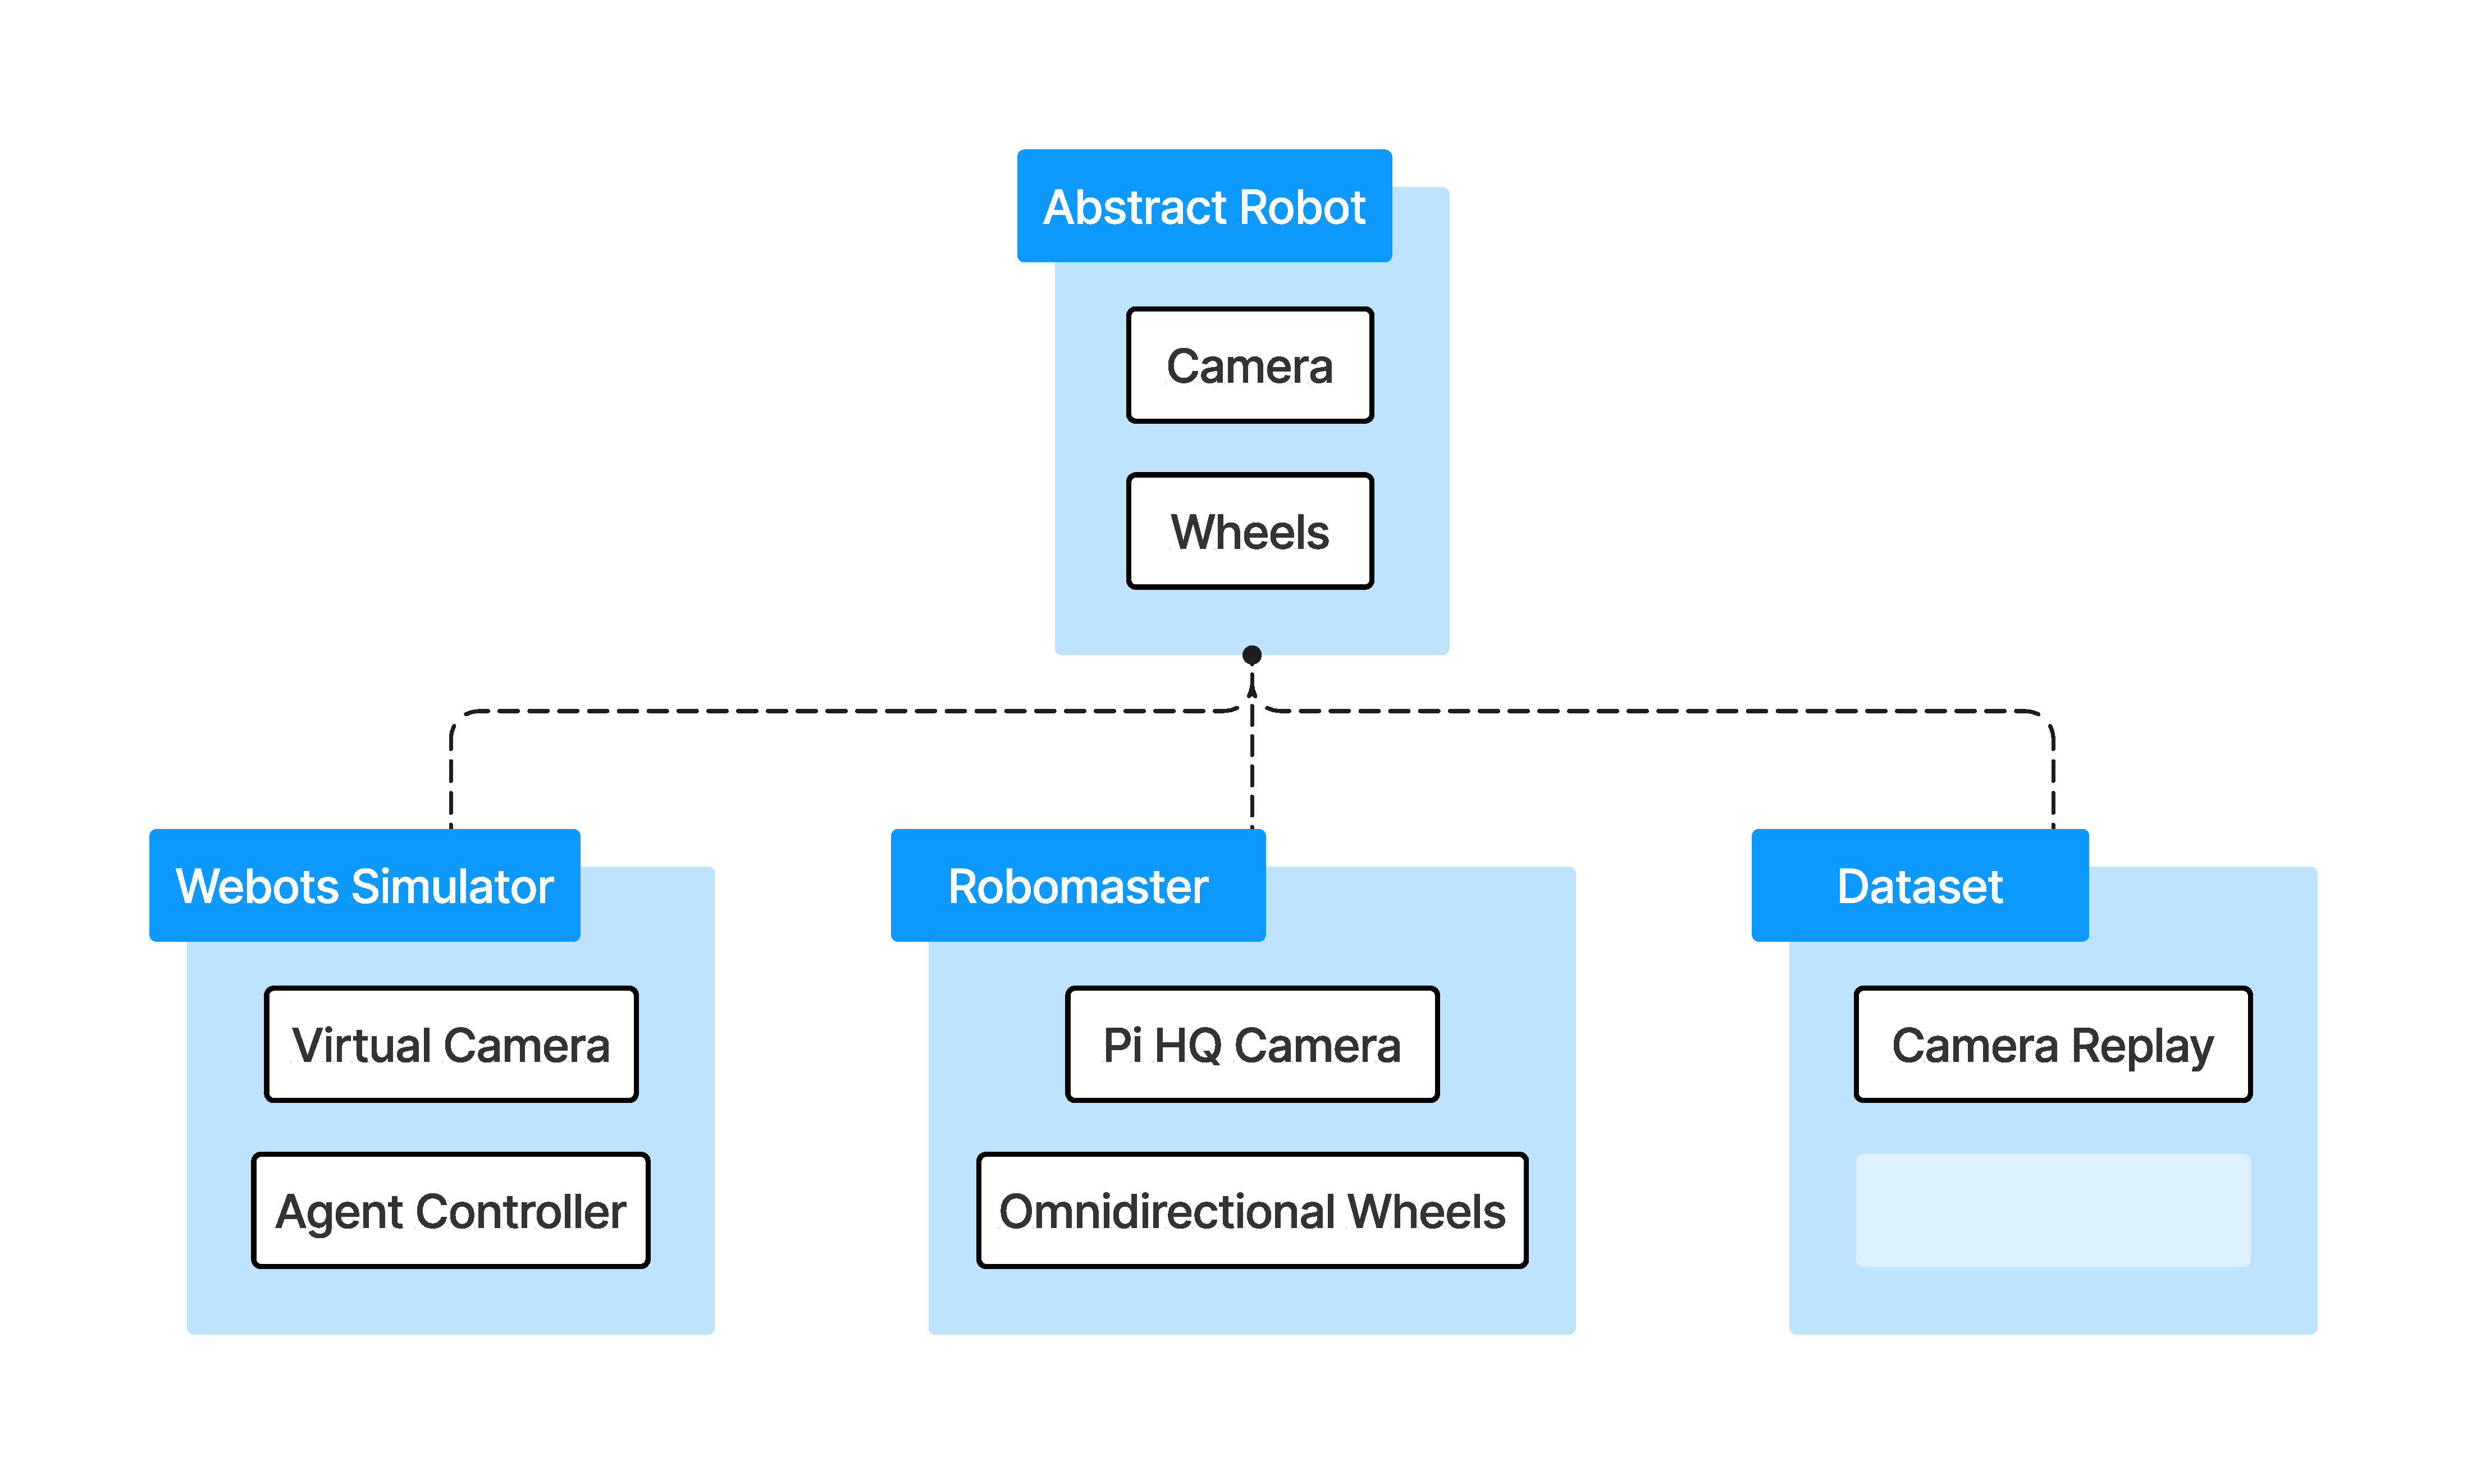
\includegraphics[trim=5cm 5cm 5cm 5cm, scale=0.2]{figures/abstract_camera_interface.pdf}

    \caption{All robot types inherit the abstract robot interface, allowing my SLAM system and its supporting infrastructure to be completely agnostic to the actual type of robot used.}
    \label{fig:abstract-camera-interface}
\end{figure}

Furthermore, using the ROS framework allows my code to be far more portable, as anyone can download my nodes, link the camera topics up to their robot's camera, and run my SLAM system with minimal effort. This turns my project from being something that only runs on my hardware to something that anyone can take and run on their own robot.

There are two versions of ROS: ROS 1 and ROS 2. I chose to use ROS 2 due to its improved decentralized properties, which align with the goals of this project. ROS 2 conforms to the Data Distribution Service (DDS)\footnote[1]{\url{https://en.wikipedia.org/wiki/Data_Distribution_Service}} specification, which guarantees a reliable broadcast and, unlike ROS 1, it does not require a leader node when used in a multi-agent setup.

TODO: clangd and build stuff?

\subsection{Docker Containers}
\label{sec:docker-containers}
Docker containers are used on all physical deployments of my software, including the Cambridge RoboMasters used for real-world testing of my SLAM system and my Raspberry Pi Video Publisher platform which is used for custom dataset collection and augmented reality visualizations.

Docker allows the software to be isolated in self-sufficient environments, making it easy to deploy on many computing environments. Additionally, using Docker allows my code to be built once and then deployed on multiple robots, preventing the need to rebuild the system on every robot which saves a significant amount of time. These aspects of Docker are expanded upon in the section below.

\subsection{Continuous Integration / Continuous Deployment}
\label{sec:cicd}
My GitHub repositories are set up to perform continuous integration via GitHub Action. Every time code is pushed to the repository, all 5 core packages (\texttt{controller}, \texttt{interfaces}, \texttt{motion\_controller}, \texttt{orb\_slam3\_ros}, \texttt{webots\_sim}) are built to ensure there are no compile time errors.

Additionally, a Docker container is cross-compiled to \texttt{arm64} and uploaded to Docker Hub. These Docker images can then be downloaded to the Cambridge RoboMasters (the platform used for real-world testing) and immediately run. This greatly speeds up development, as compiling the codebase locally on the Cambridge RoboMasters takes over 20 minutes for each robot.

Aside from the core packages, we also perform continuous integration as well as continuous deployment for the Raspberry Pi video publisher package. This pipeline is displayed in \autoref{fig:cicd-diagram}. A Docker container is similarly cross-compiled to \texttt{arm64} and uploaded to Docker Hub, and it is automatically deployed to the Raspberry Pis so they will run the latest version of the package.

Continuous deployment makes sense for this use case as the Raspberry Pis are designed to be plug-and-play, starting video streaming as soon as they are turned on. Unlike the Cambridge RoboMasters which are frequently ssh'ed into to pull specific Docker images and start experiments, we want the Raspberry Pis to use the latest software as soon as it is pushed to the GitHub repository.

The ease of use of the Raspberry Pi ROS video publisher platform that I have developed has made them an invaluable tool in the Prorok Lab, even being used by other researchers. TODO: get other people to use them lol

\begin{figure}[h]
    \centering
    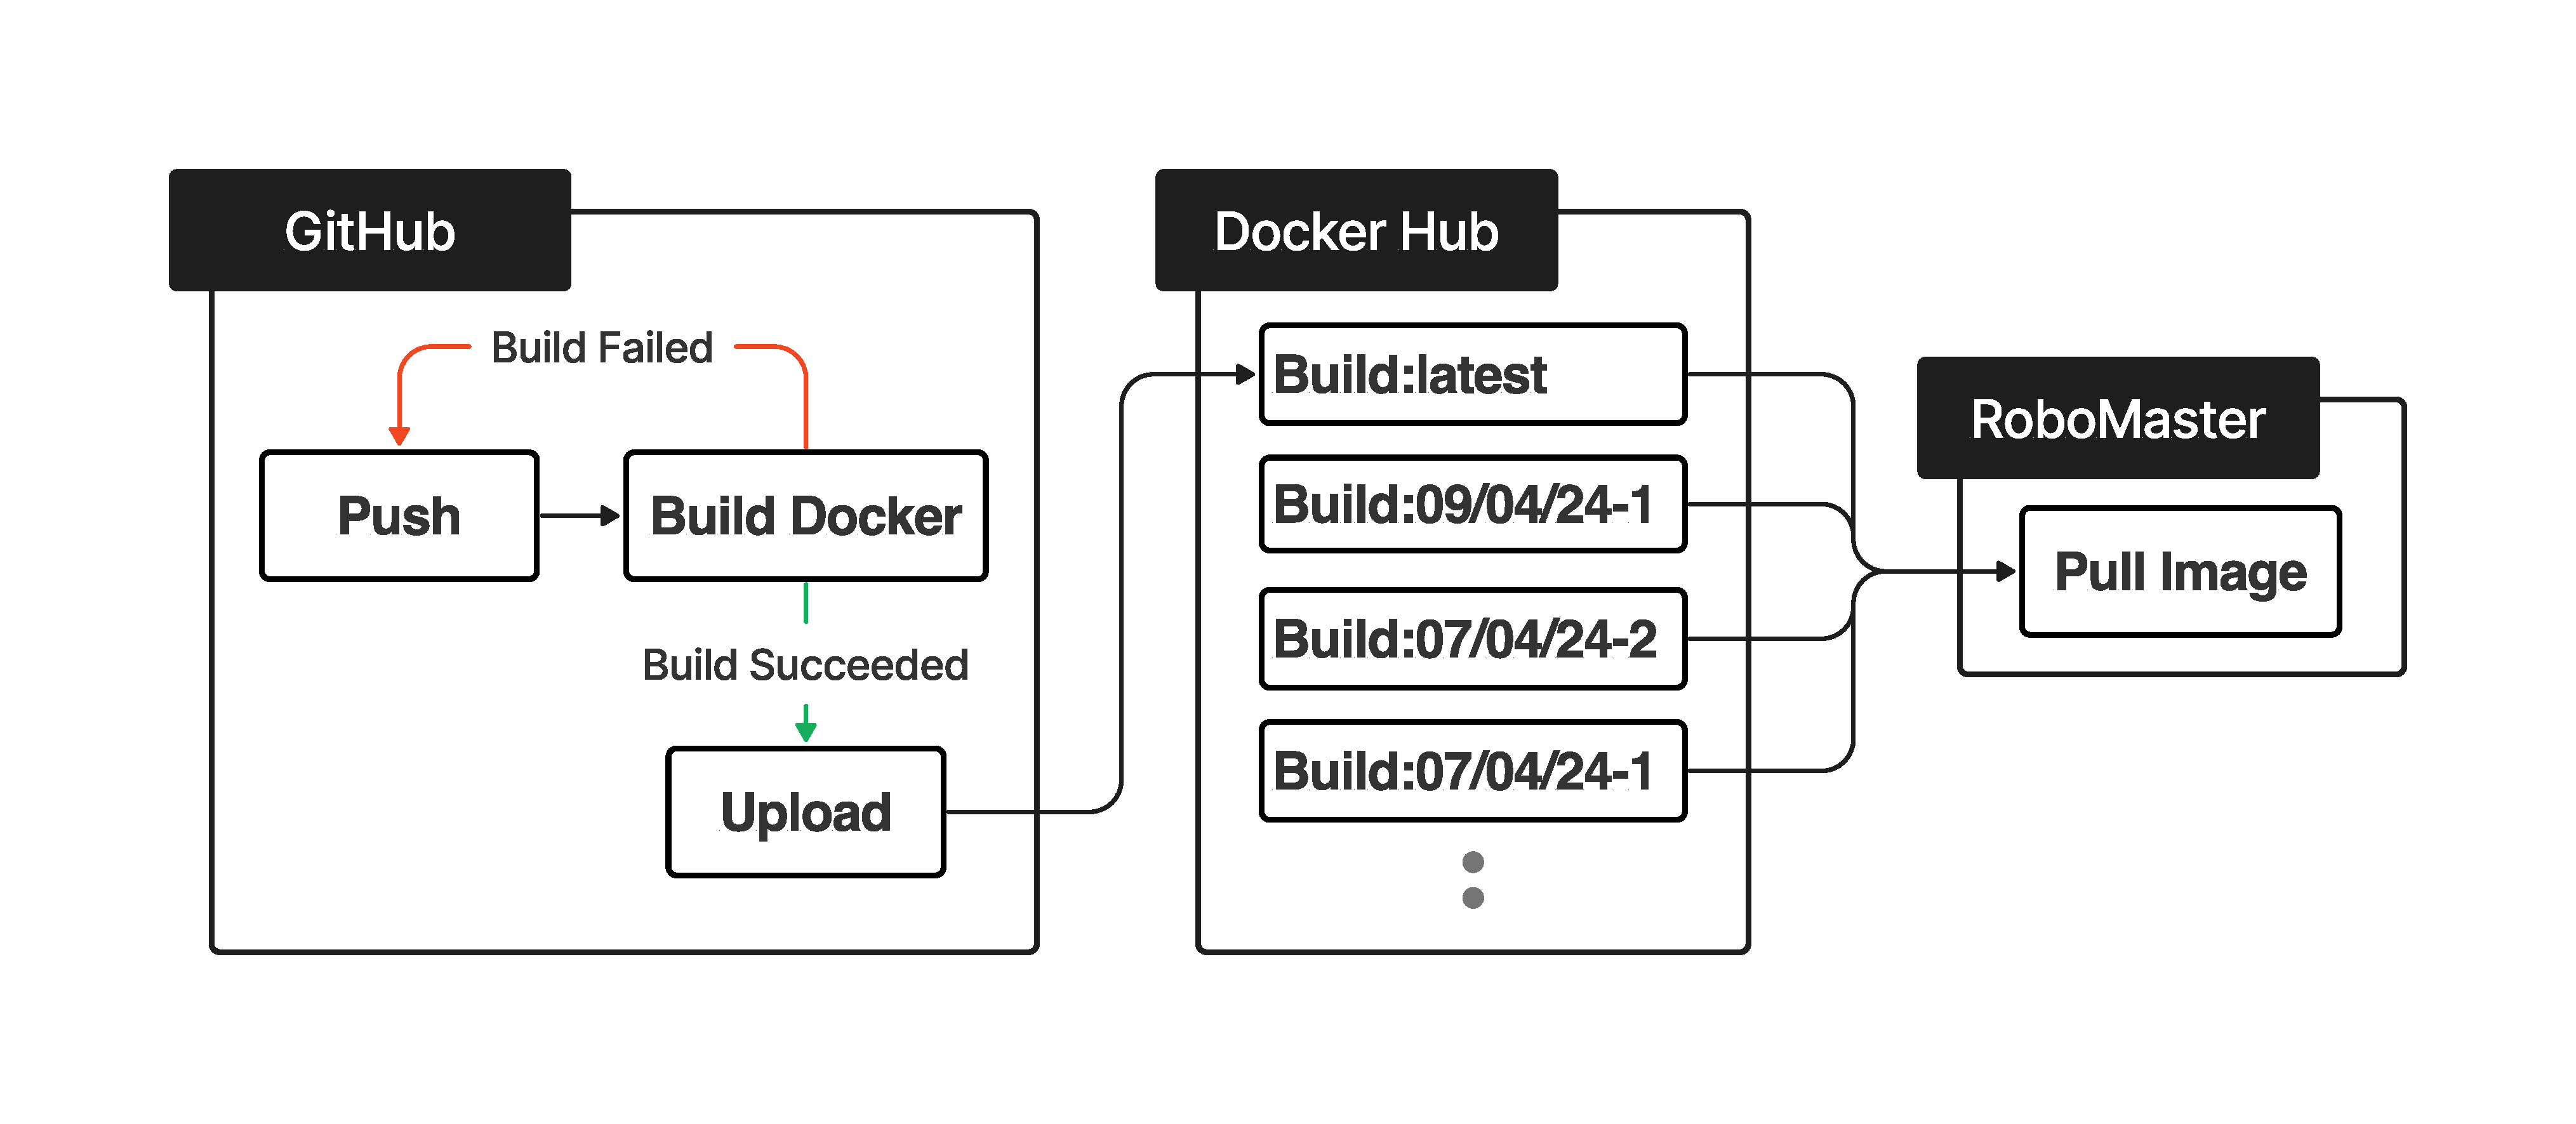
\includegraphics[trim=5cm 5cm 5cm 5cm, scale=0.2]{figures/cicd_diagram.pdf}

    \caption{Automated continuous integration pipeline for the Cambridge RoboMasters. Continuous deployment is implemented for the Raspberry Pi video publishers by pulling from Docker Hub and running the container on startup.}
    \label{fig:cicd-diagram}
\end{figure}


\section{Datasets}
\label{sec:datasets}
A variety of industry-standard datasets were utilized to benchmark the performance of my SLAM system, including the EuRoC Machine Hall \autocite{burri2016euroc} and TUM-VI \autocite{8593419} datasets. While these datasets provide a variety of sensors, we only utilize a monocular video as input when evaluating performance. Further information about each dataset is provided in the \nameref{sec:benchmarking} section.

In addition to standard datasets, I also generated custom datasets within the simulated environment to use as regression tests during development. These datasets test individual capabilities of the system such as multi-agent map merging, losing localization, etc. I then ran these tests on my system to ensure that the system performed as expected and that metrics such as time-to-merge and average trajectory error were decreasing as I iterated on my system.

\section{Algorithms}
\label{sec:algorithms}
This section will briefly cover some of the existing algorithms utilized within my SLAM system, and can be used as a reference when reading the \nameref{sec:3} section.

\subsection{Kabsch-Umeyama Algorithm}
\label{sec:kabsch-umeyama-algorithm}

\subsection{Visual Bag of Words}
\label{sec:visual-bag-of-words}

\subsection{RANSAC}
\label{sec:ransac}

\section{Requirements Analysis}
\label{sec:requirements-analysis}

\subsection{Development Model}
\label{sec:development-model}

